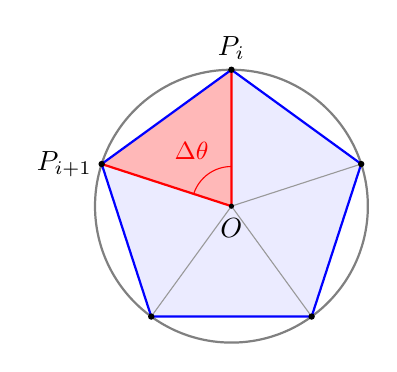
\begin{tikzpicture}[scale=1.05]
  \def\R{1.65}
  \draw[gray, thick] (0,0) circle (\R);
  \coordinate (O) at (0,0);
  \foreach \k in {0,1,2,3,4} {
    \coordinate (V\k) at ({90+72*\k}:\R);
  }
  \fill[blue!8] (V0)--(V1)--(V2)--(V3)--(V4)--cycle;
  \fill[red!28] (O)--(V0)--(V1)--cycle;
  \draw[blue, thick] (V0)--(V1)--(V2)--(V3)--(V4)--cycle;
  \draw[gray!80] (O)--(V2) (O)--(V3) (O)--(V4);
  \draw[red, thick] (O)--(V0) (O)--(V1);
  \fill (O) circle (0.9pt) node[below=1pt] {$O$};
  \foreach \k in {0,1,2,3,4} {\fill (V\k) circle (1.1pt);}
  \node[above] at (V0) {$P_i$};
  \node[left] at (V1) {$P_{i+1}$};
  \draw[red] (90:0.48) arc (90:162:0.48);
  \node[red, font=\small] at (126:0.82) {$\Delta\theta$};
\end{tikzpicture}
